\documentclass[border=0.2cm]{standalone}
\usepackage{tikz}
\usetikzlibrary{automata, positioning}

\title{fsm}

\begin{document}
    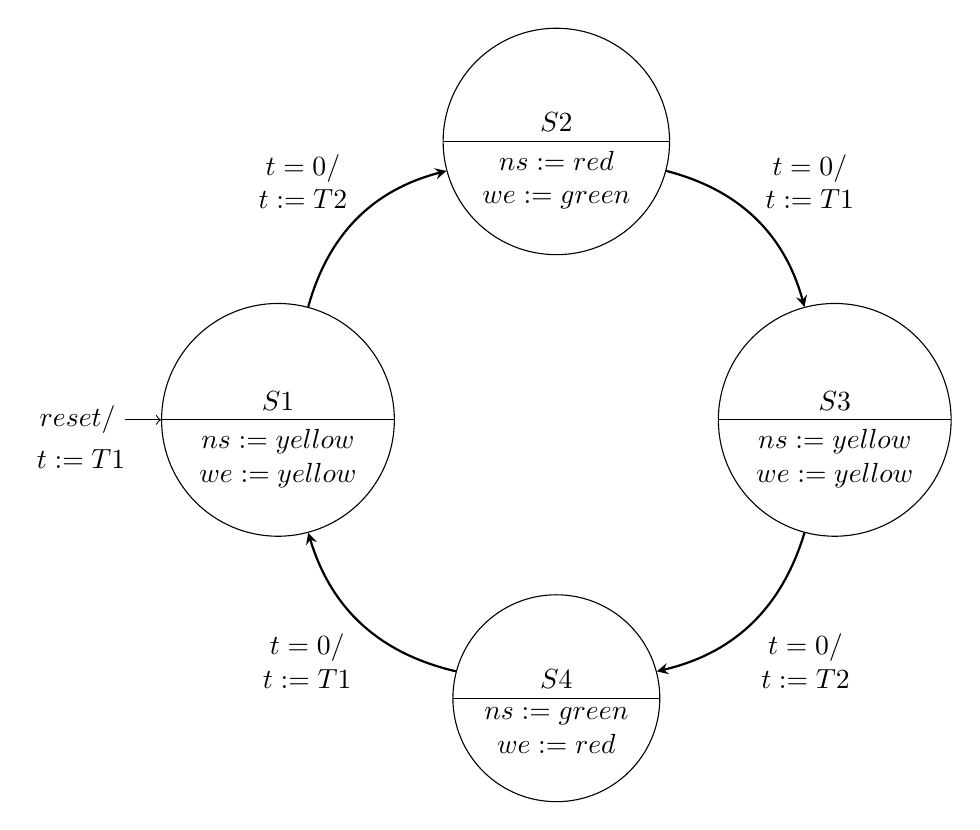
\begin{tikzpicture} [node distance = 5cm, on grid, auto]
        \node (s1)
        [state with output, initial left, initial text = {$reset/$}, align=center]
        {$S1$ \nodepart{lower} $ns:=yellow$\\$we:=yellow$};
        \node (s2)
        [state with output, above right = of s1, align=center]
        {$S2$ \nodepart{lower} $ns:=red$\\$we:=green$};
        \node (s3)
        [state with output, below right = of s2, align=center]
        {$S3$ \nodepart{lower} $ns:=yellow$\\$we:=yellow$};
        \node (s4)
        [state with output, below left = of s3, align=center]
        {$S4$ \nodepart{lower} $ns:=green$\\$we:=red$};

        \path [-stealth, thick]
        (s1) edge [bend left] node [align=center] {$t=0/$\\$t:=T2$} (s2)
        (s2) edge [bend left] node [align=center] {$t=0/$\\$t:=T1$} (s3)
        (s3) edge [bend left] node[align=center] {$t=0/$\\$t:=T2$} (s4)
        (s4) edge [bend left] node[align=center] {$t=0/$\\$t:=T1$} (s1)
        ;
        \node[align=left] at (-2.5,-0.5) {$t:=T1$};
    \end{tikzpicture}
\end{document}